\documentclass[a4paper,10pt]{report}
\usepackage[utf8]{inputenc}
\usepackage{graphicx}

% Title Page
\title{tp coloration}
\author{Arnaud Cojez \and Matthieu Caron}


\begin{document}

\maketitle

\section{Structure de Donnée utilisée}
Pour notre représentation de graphe on a trois classes différente,
\begin{itemize}
 \item la classe Sommet qui contient la liste des Aretes qui lui sont associés et une couleur.
 \item la classe Arete qui contient deux sommets
 \item la classe Graph qui contient la liste de toutes les aretes ainsi que la liste de tous les sommets.
\end{itemize}

\section{Les Algorithmes de coloriage}
les algoritmes choisi sont les suivants : l'algoritme naif, l'algoritme DSATUR et l'algoritme de Welsh Powel.

\begin{center}
  \begin{figure}[h]
    \label{color}
    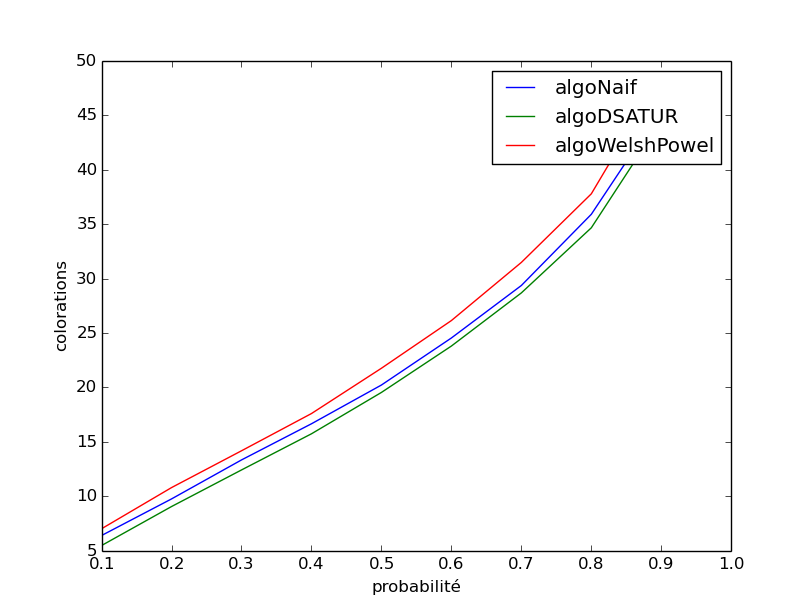
\includegraphics[scale=0.5]{coloration.png}
    \caption{Nombre de couleur en fonction de p}
  \end{figure} 
\end{center}

\begin{center}
  \begin{figure}[h]
    \label{time}
    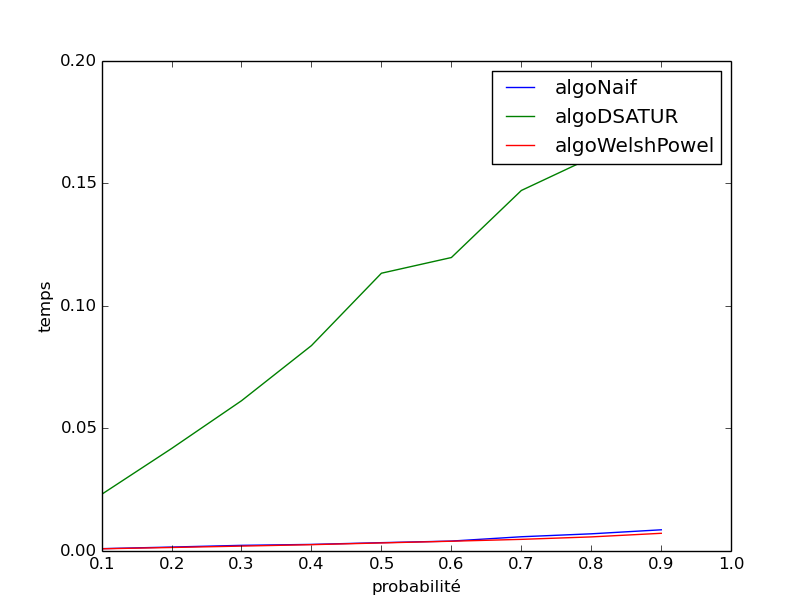
\includegraphics[scale=0.3]{temps.png}
    \caption{Temps de calcul en fonction de p}
  \end{figure} 
\end{center}




\end{document}          
